\chapter{Concurrent Objects}

\section{Concurrent Queues}
We start with a basic interface defining the behaviour of a queue.
\begin{minted}{Kotlin}
interface Queue<T> {
    val count: Int
        get
    
    val isEmpty: Boolean
        get() = count == 0

    fun enq(item: T): Boolean
    fun deq(): T?
} 
\end{minted}

\subsection{Circular Queue}
\begin{minted}{kotlin}
class CircularQueue<T>(val capacity: Int) : Queue<T> {
    var head: Int = 0  // next pop present here
    var tail: Int = 0  // next item pushed here
    var items = MutableList<T?>(capacity){null}
    
        override val count: Int
        get() = if  (head >= tail) head - tail else head + (capacity - tail)
    
    override fun enq(item: T): Boolean {
        if (count < capacity) {
            items[head] = item    
            head = (head + 1) % capacity
            return true
        } else {
            return false
        }
    }
    
    override fun deq(): T? {
        if (isEmpty) {
            return null
        } else {
            val retval: T = items[tail]!!
            tail = (tail + 1) % capacity
            return retval
        }
    }
}
\end{minted}

\subsection{Lock Based Queue}
Mutual exclusion is used to prevent concurrent modification, and hence make thread safe.
\begin{minted}{Kotlin}

\end{minted}

\subsection{Wait Free 2-Thread Queue}

\unfinished

\section{Sequential and Concurrent Objects}
\begin{definitionbox}{Object}
    Objects are data structures containing internal state (fields/attributes/members) and methods (functions that can be provided input, and access/mutate the object's internal state).
\end{definitionbox}
In concurrent programming, the liveness and safety properties of an object must be specified.
\begin{itemize}
    \item Need to define how to assess the implementation as correct
    \item Need to define under which conditions progress (e.g no livelock/deadlock) is guaranteed
\end{itemize}

\subsection{Sequential Specifications}
\begin{center}
    \begin{tabular}{l p{.8\textwidth}}
        \textbf{Precondition} & Object state before method call \\
        \textbf{Postcondition} & (Result) Value returned by the method, or exceptions thrown \\
        \textbf{Postcondition} & (State)  The state of the object when the method returns \\
    \end{tabular}
\end{center}
We do not need to consider the state of the object between the rep and post conditions.
\begin{itemize}
    \item State is meaningful between method calls (postcondition (state) $\to$ precondition)
    \item Each method call can be considered a single atomic event
    \item Methods can be described in isolation
    \item New methods can be added without changing the descriptions of older methods
\end{itemize}

\subsection{Concurrent Specifications}
A method call is no longer an atomic event.
\begin{itemize}
    \item A method call is a sequence of interval events.
    \item Method calls overlap in time.
    \item Object may never be \textit{between method calls} as many calls may constantly overlap
    \item All interactions between concurrent calls must be characterised
    \item When adding a new method, it must be considered in the context of all existing method definitions 
    \item \textbf{everything can interact with everything else}
\end{itemize}

\begin{definitionbox}{Linearisable}
    A set of operations are linearisable if it can be re-expressed as a sequential history.
\end{definitionbox}

\begin{tcbraster}[raster columns=2,raster equal height]
    \begin{definitionbox}{Object Linearisability}
        An object is linearisable if all its possible executions are linearisable.
        \\
        \\
        \\ \textit{Not studied in this course}  
    \end{definitionbox}
    \begin{definitionbox}{Execution Linearisability}
        \begin{itemize}
            \item Method takes effect instantaneously somewhere between the invocation and response events.
            \item If the \textit{sequential} behaviour is correct then the execution is linearisable.
        \end{itemize}
    \end{definitionbox}
\end{tcbraster}
\begin{center}
    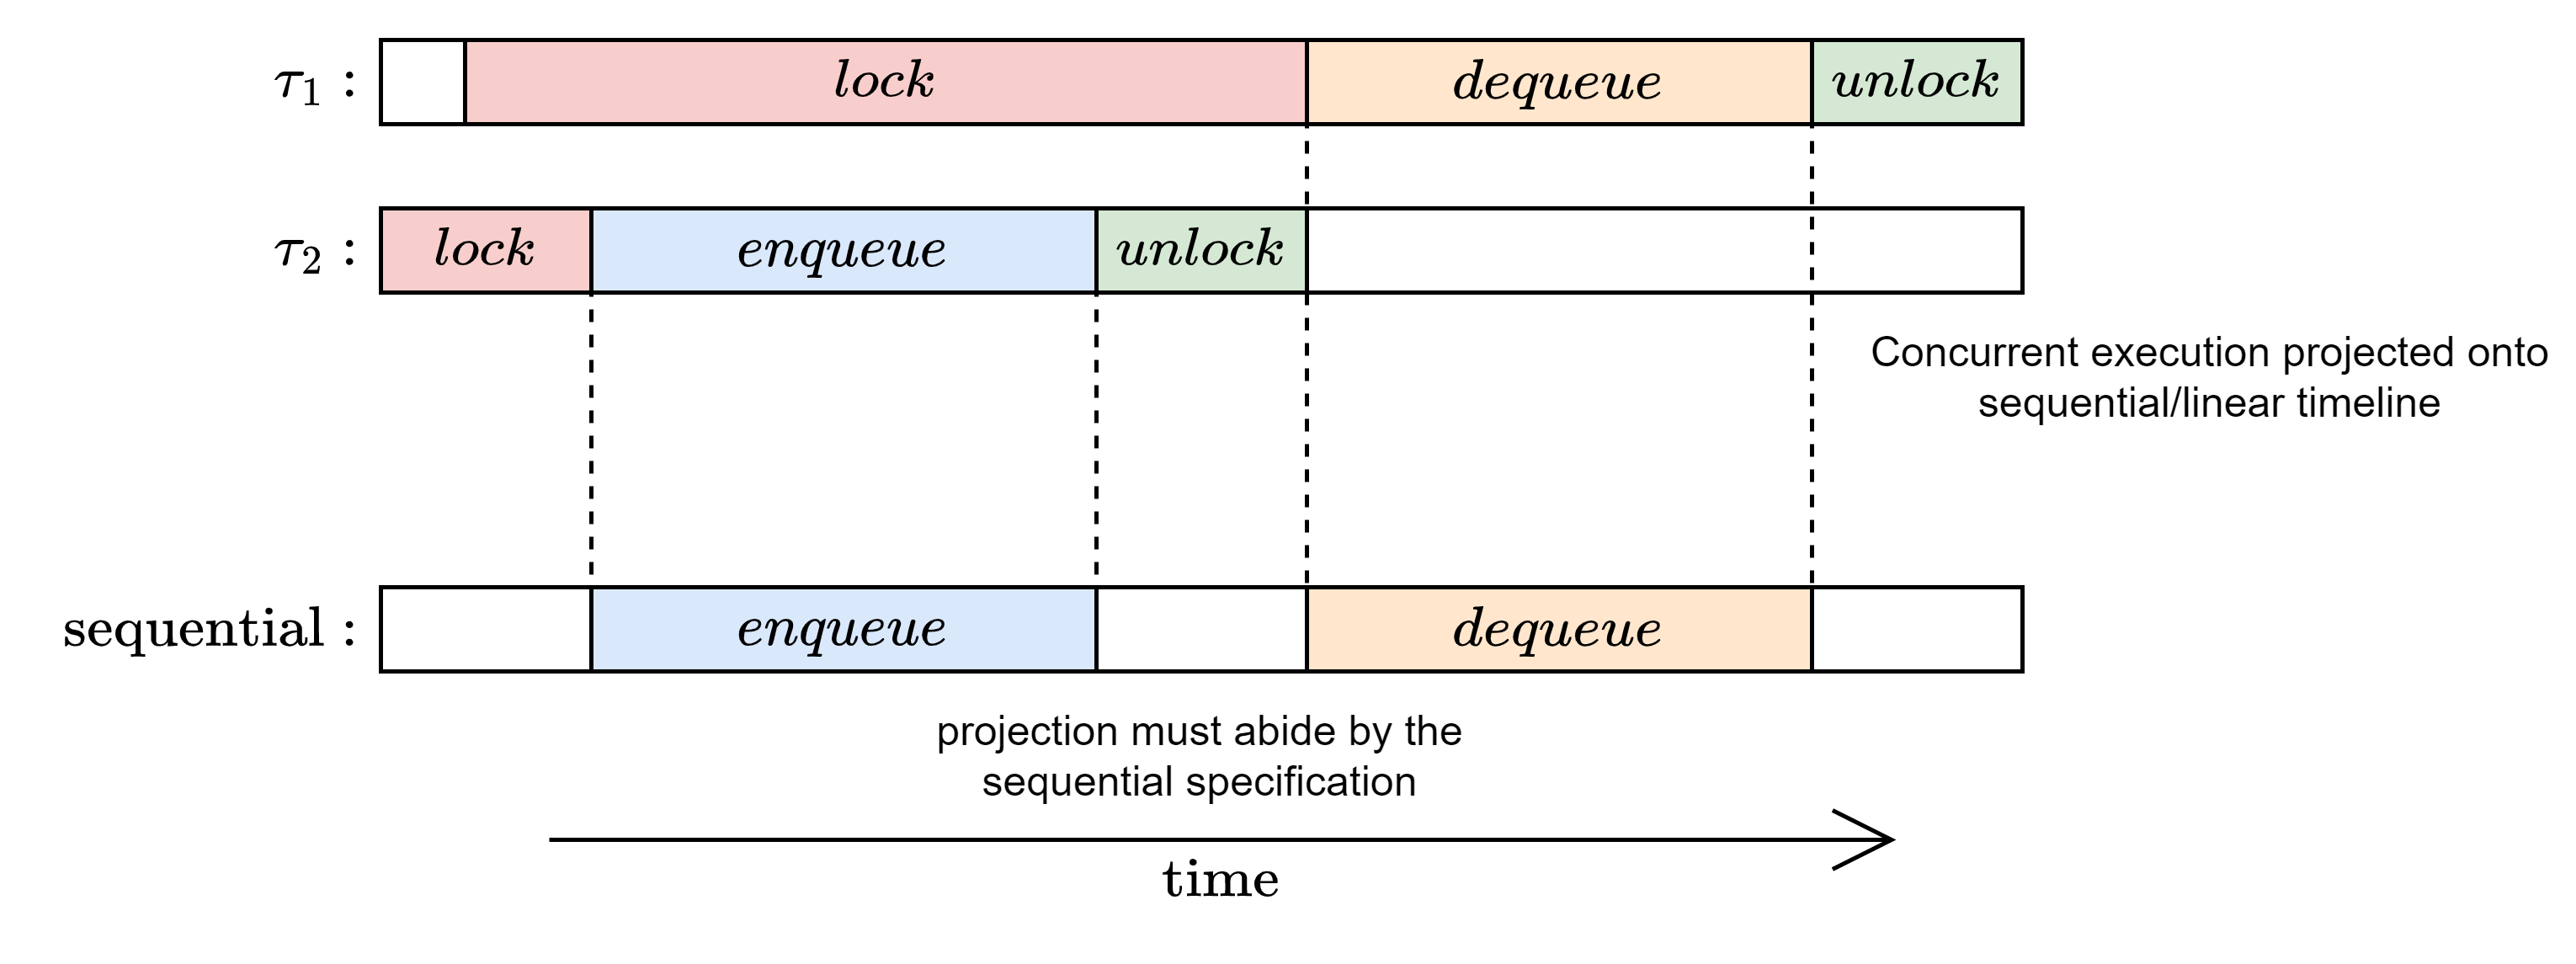
\includegraphics[width=\textwidth]{concurrent_objects/images/sequential_projection.drawio.png}
\end{center}
\begin{itemize}
    \item To show an execution is linearisable, we find the linearization points (where the method \textit{instantaneously} occurs)
    \item Typically arrows are used, where a bold arrow shows the time for the execution of some method, and an arrow with a dotted tail is one that never responds/returns (e.g thread killed).
    \item For invocations that never respond/return, we can decide if the method occurred or not (depending on what \textit{makes sense}/is required to justify the execution).
\end{itemize}

\begin{examplebox}{Valid Linearisations}
    Determine the valid linearisation for the following execution.
    \begin{center}
        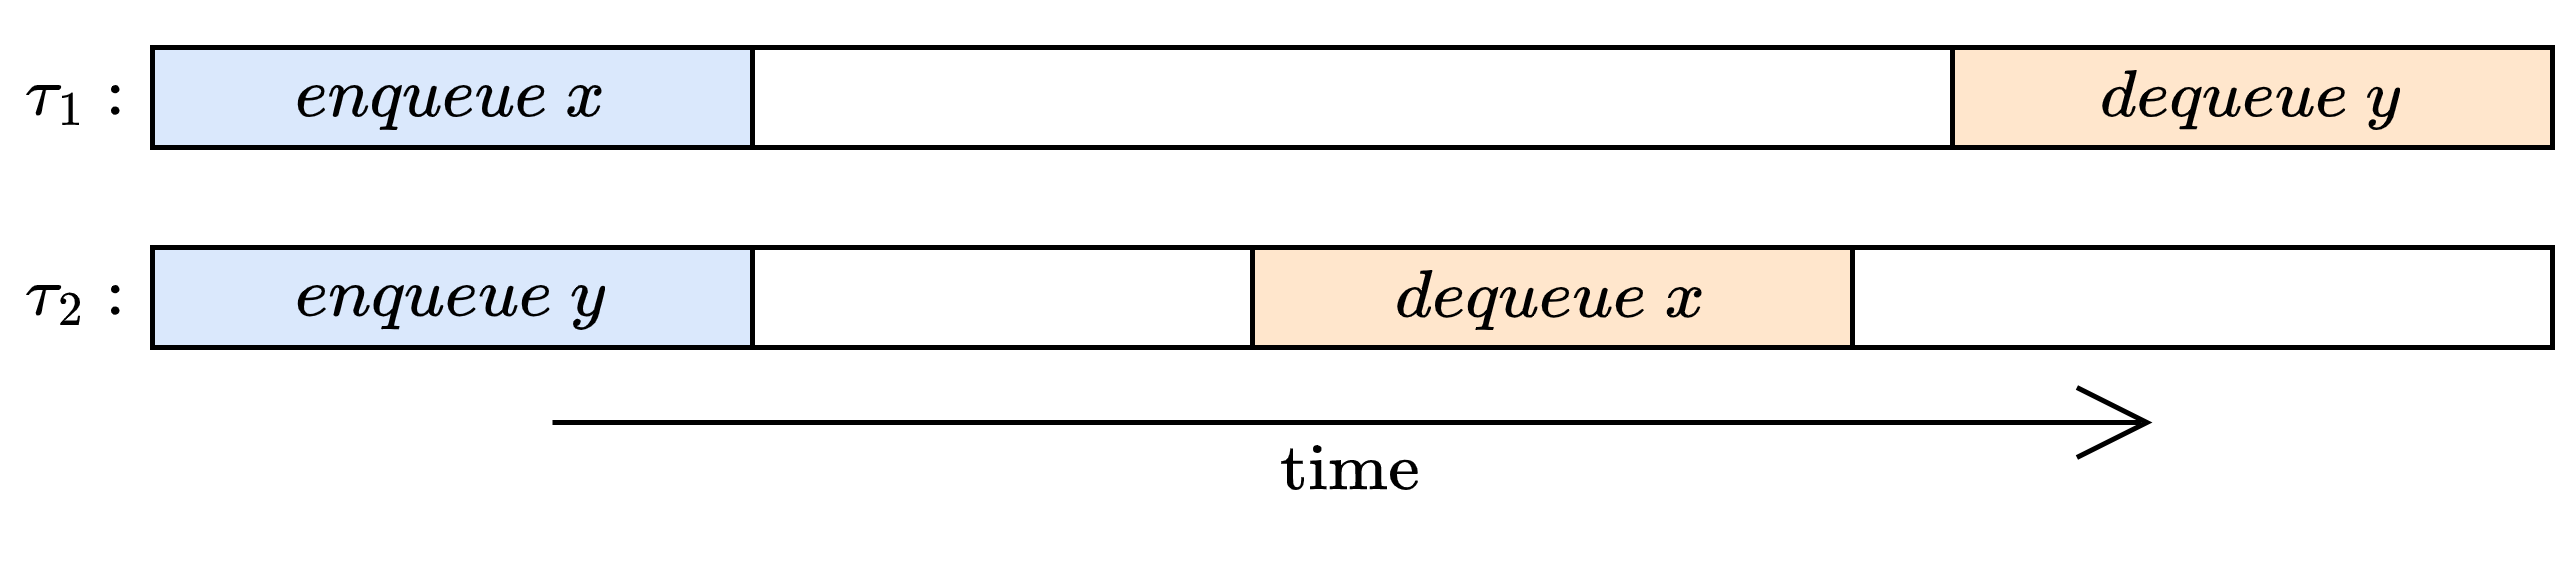
\includegraphics[width=.9\textwidth]{concurrent_objects/images/example_valid_linearisation.drawio.png}
    \end{center}
    \tcblower
    \begin{center}
        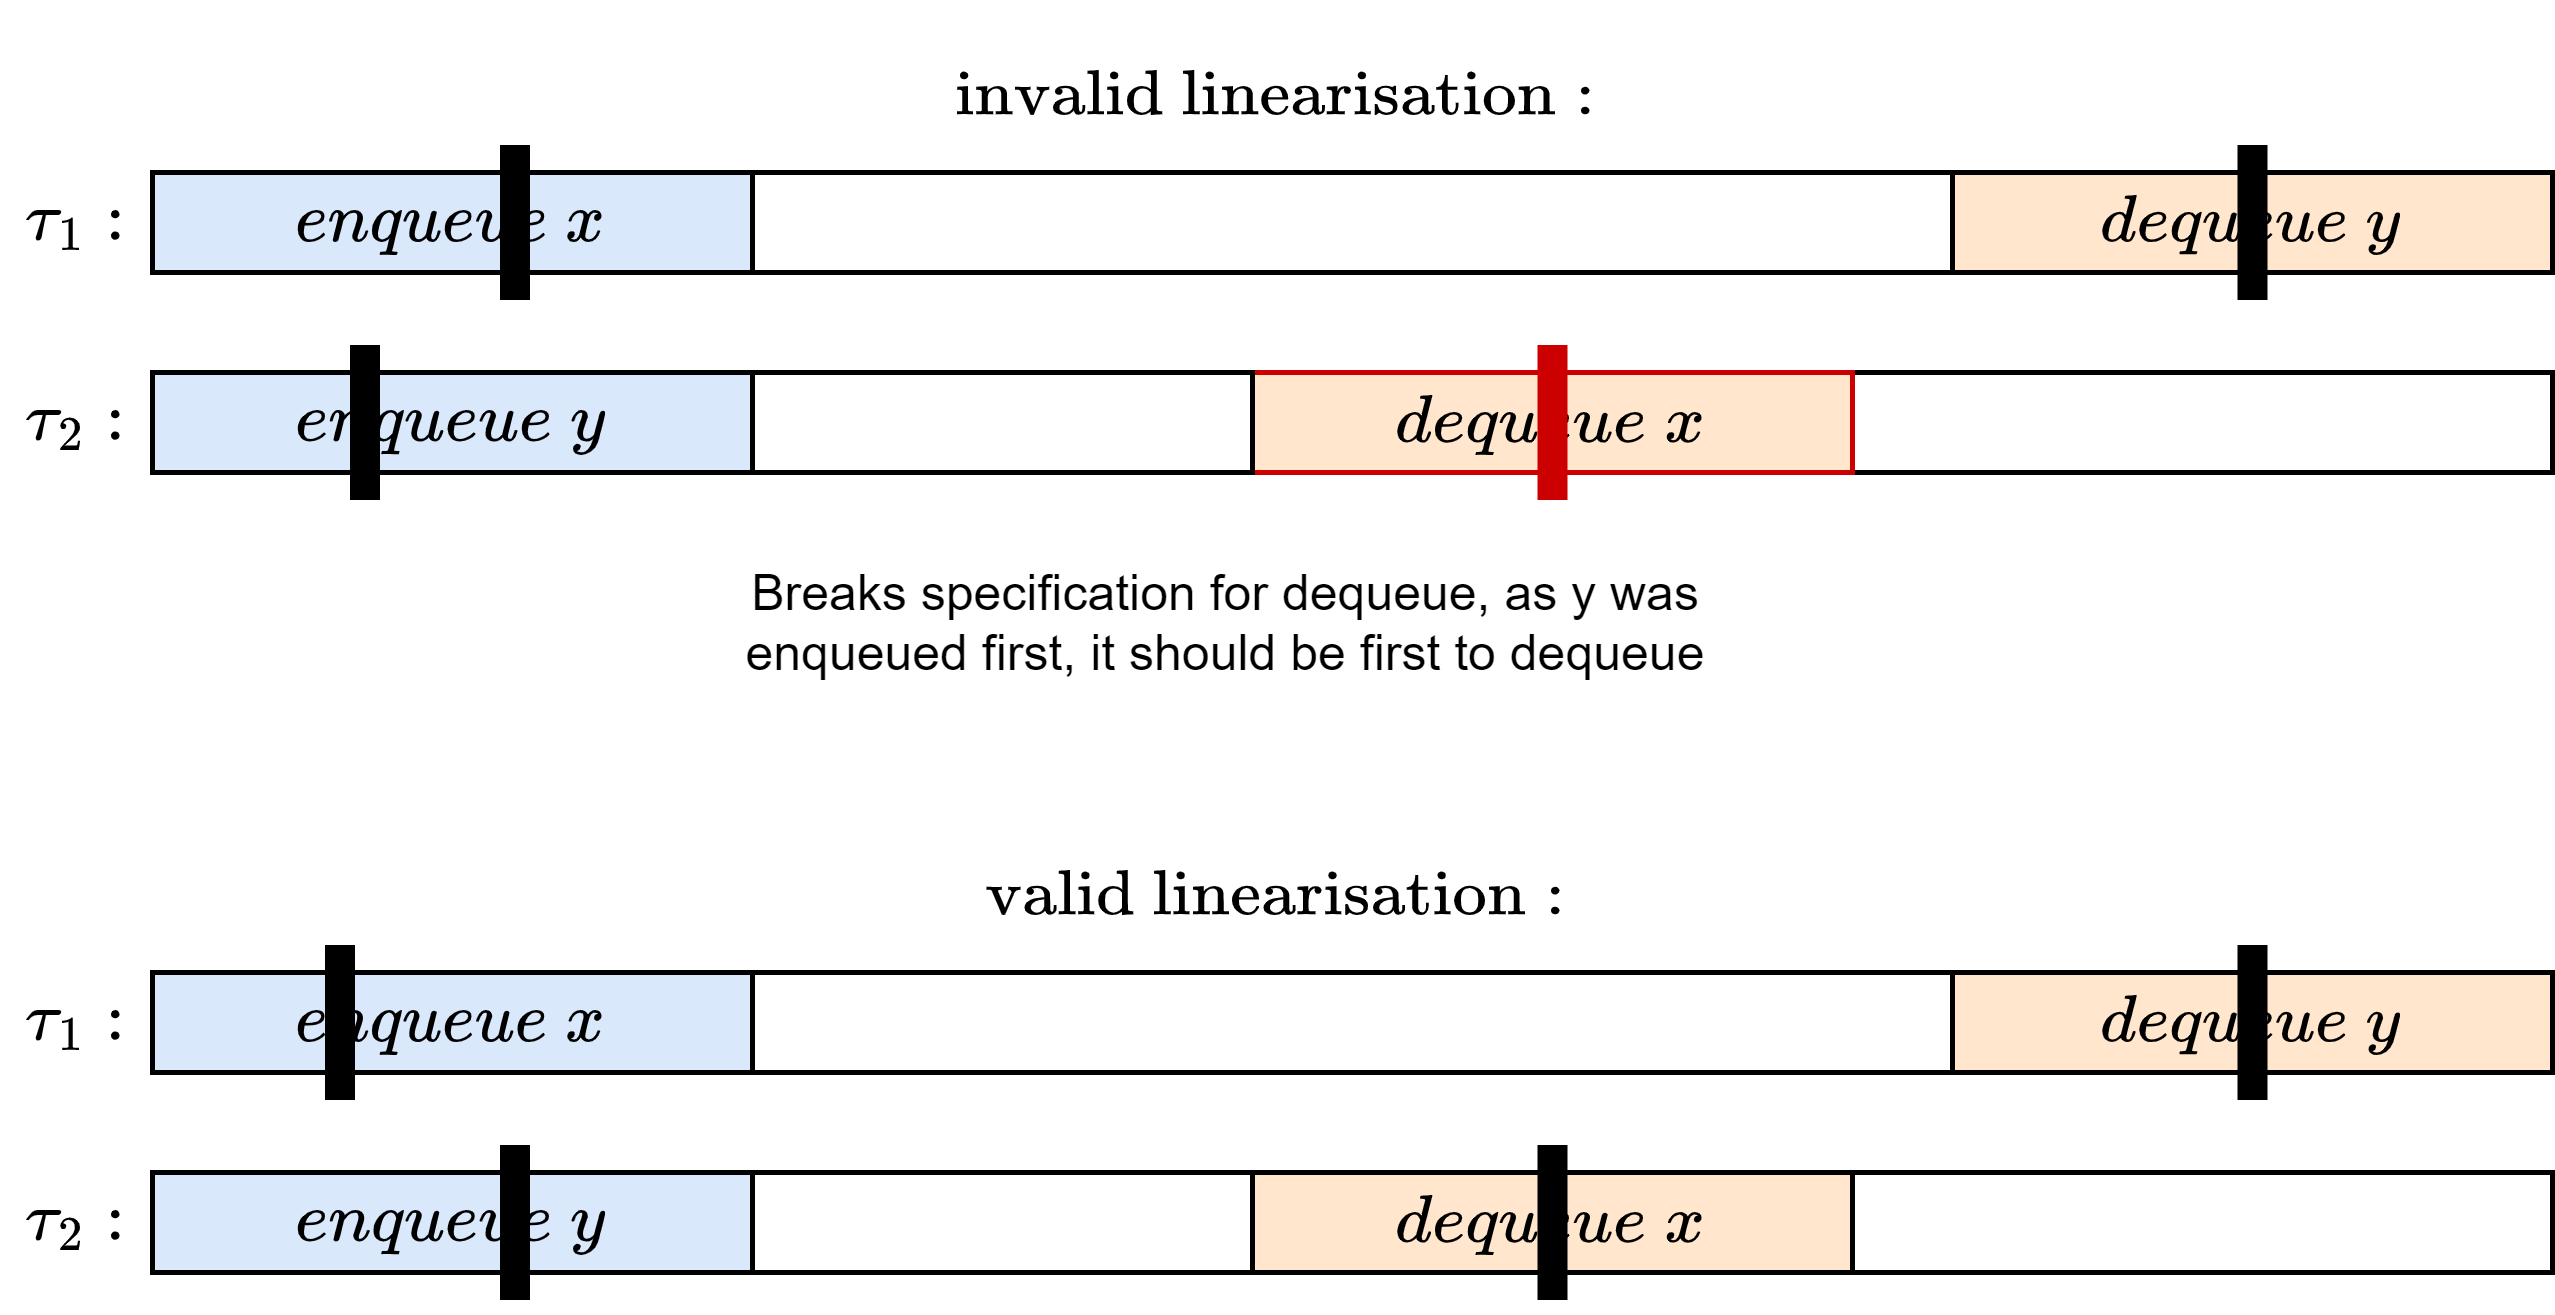
\includegraphics[width=.9\textwidth]{concurrent_objects/images/example_valid_linearisation_answer.drawio.png}
    \end{center}
\end{examplebox}

\begin{examplebox}{Valid Linearisation}
    Determine if there is a valid linearisation for the following execution.
    \begin{center}
        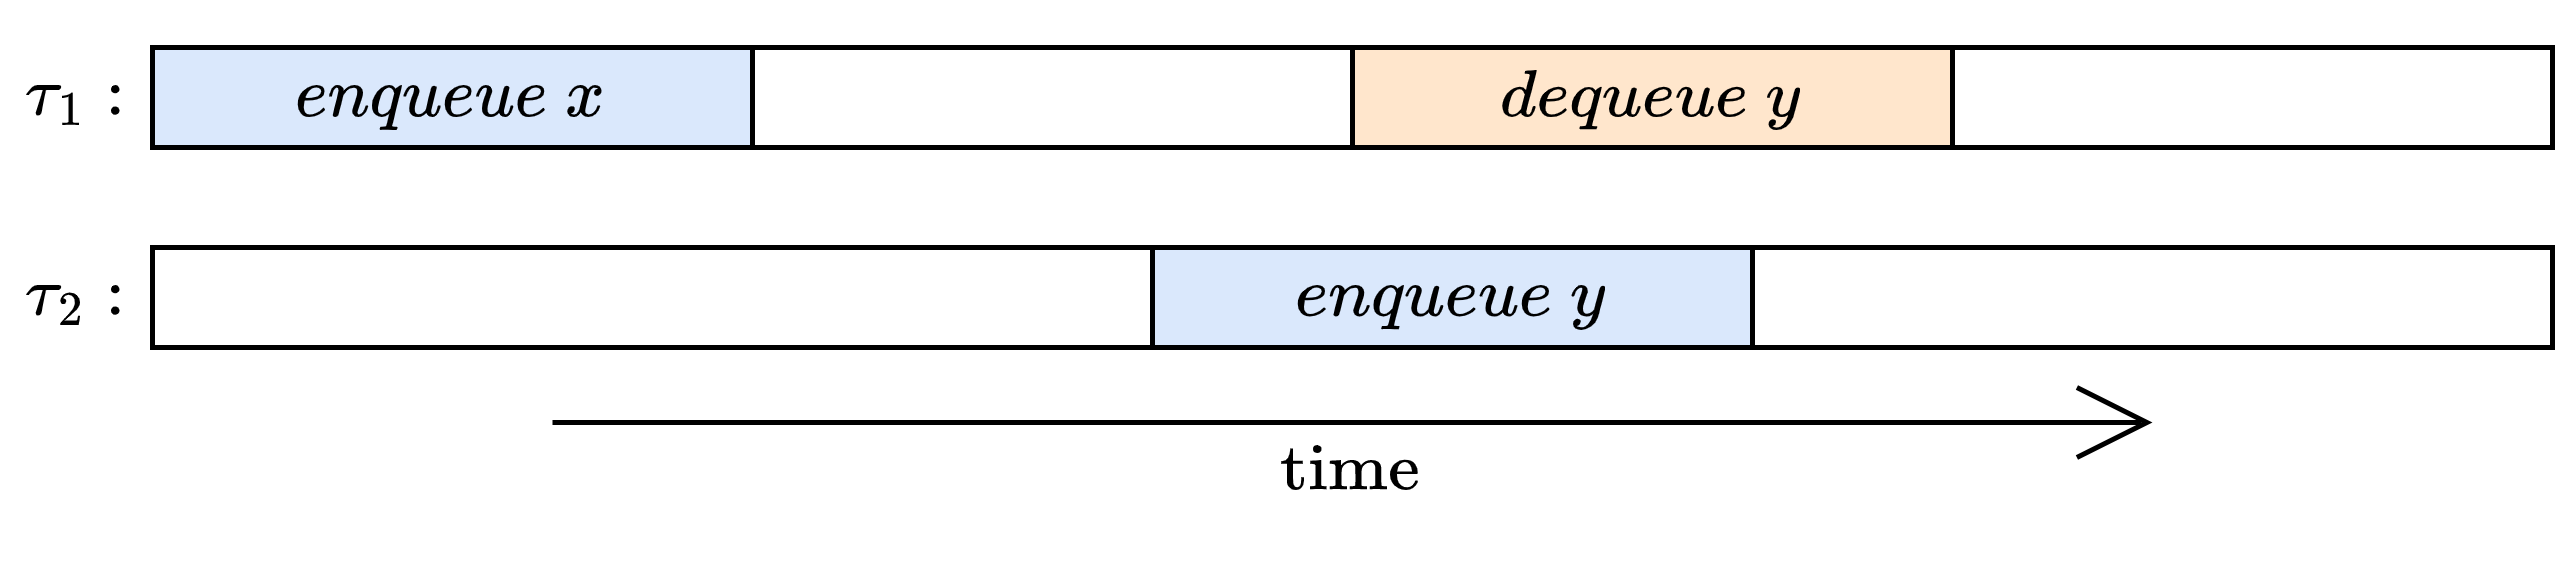
\includegraphics[width=.9\textwidth]{concurrent_objects/images/example_invalid_linearisation.drawio.png}
    \end{center}
    \tcblower
    There is none, this is as the entry to $enqueue \ x$ is before the entry to $enqueue \ y$, hence in any linearisation $enqueue \ x$ comes first. This means that the $dequeue \ y$ breaches the specification of dequeue.
\end{examplebox}

\begin{examplebox}{No Return}
    Is the following linearisable?
    \begin{center}
        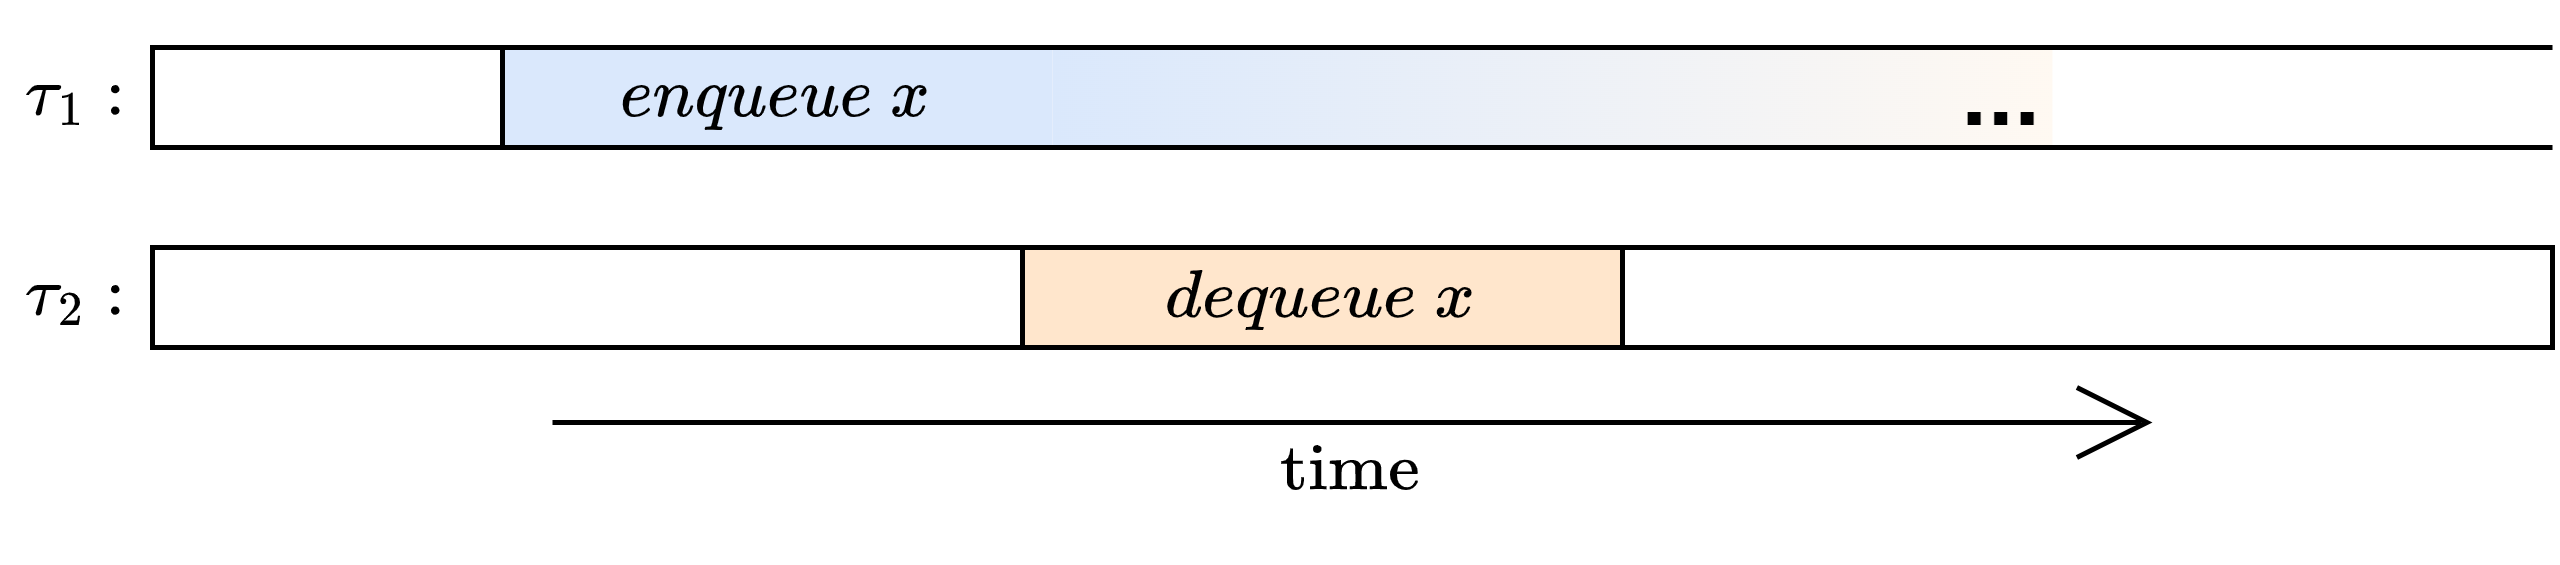
\includegraphics[width=.9\textwidth]{concurrent_objects/images/example_linearisation_no_return.drawio.png}
    \end{center}
    \tcblower
    \begin{center}
        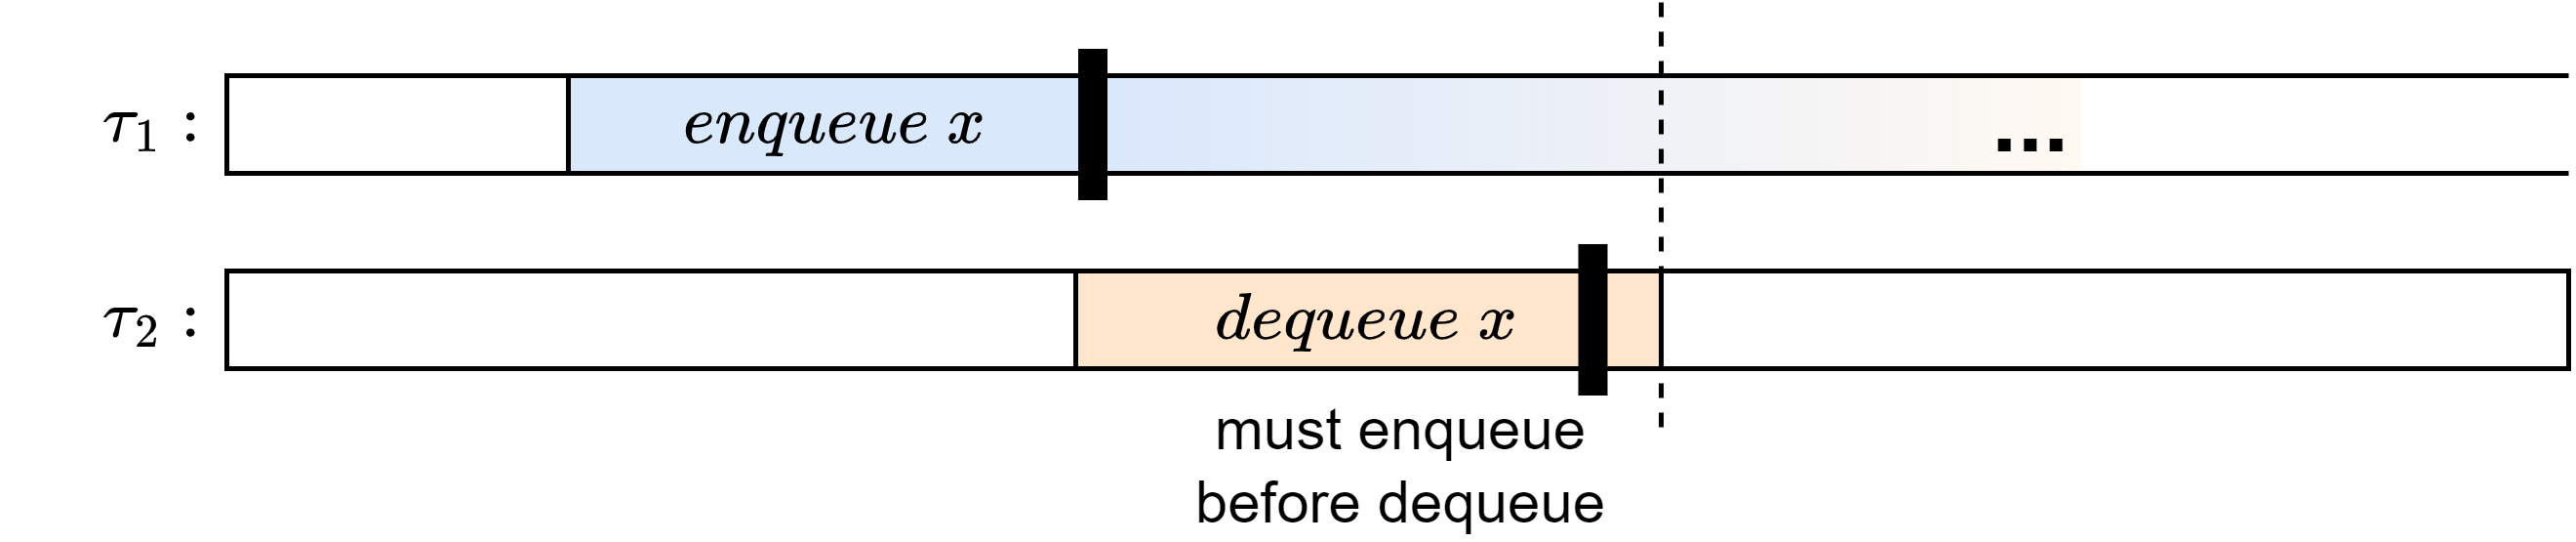
\includegraphics[width=.9\textwidth]{concurrent_objects/images/example_linearisation_no_return_answer.drawio.png}
    \end{center}
\end{examplebox}

\begin{examplebox}{Register Writing}
    Is the following execution linearisable, and if not then provide modified examples of how it could be linearisable.
    \begin{center}
        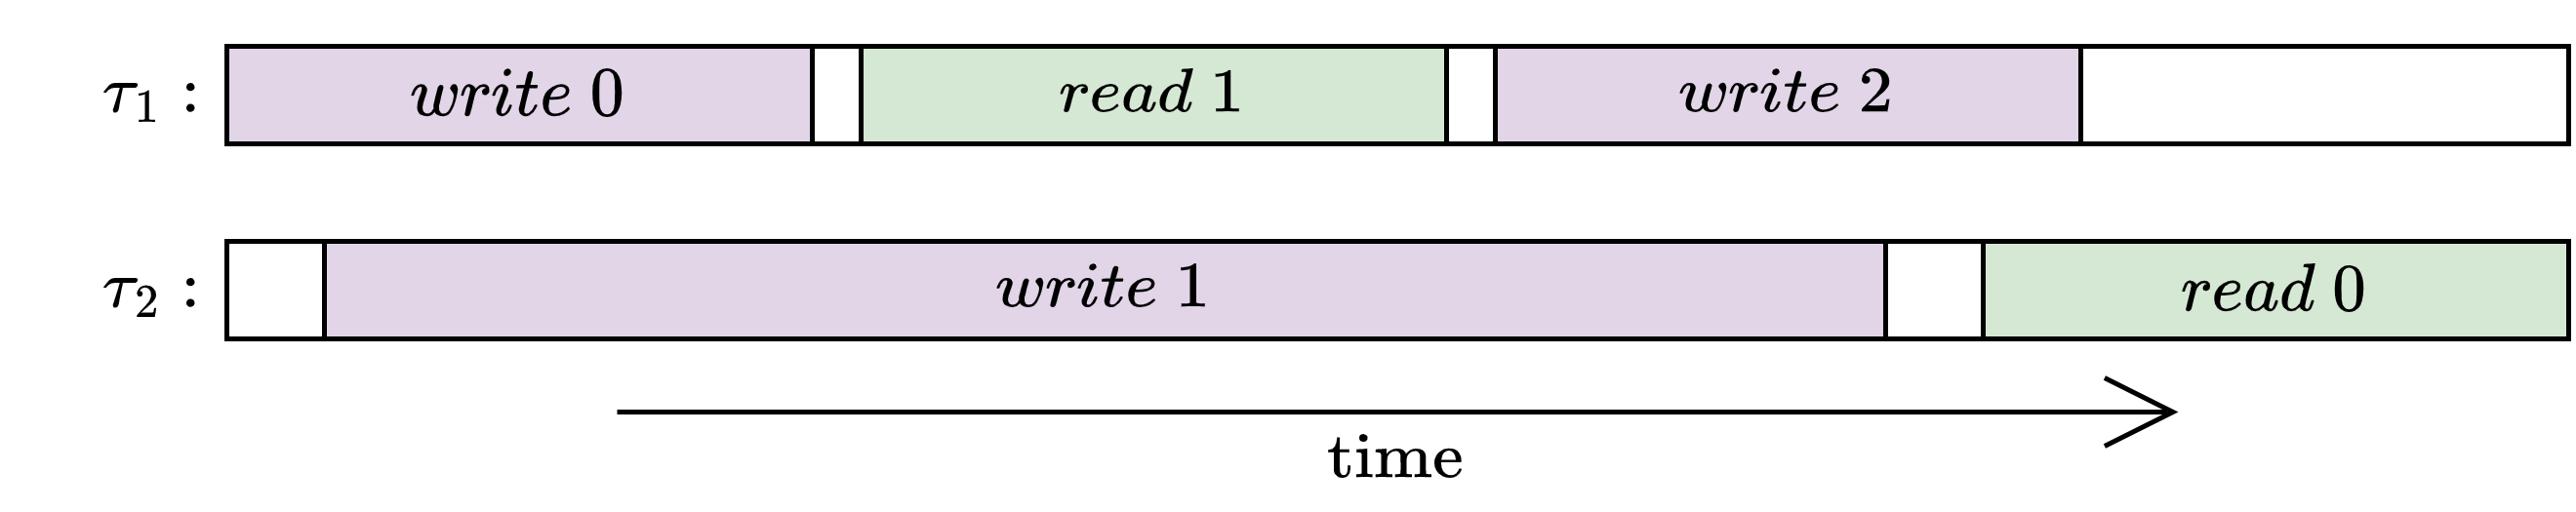
\includegraphics[width=.9\textwidth]{concurrent_objects/images/example_registers_linearisable.drawio.png}
    \end{center}
    \tcblower
    \begin{center}
        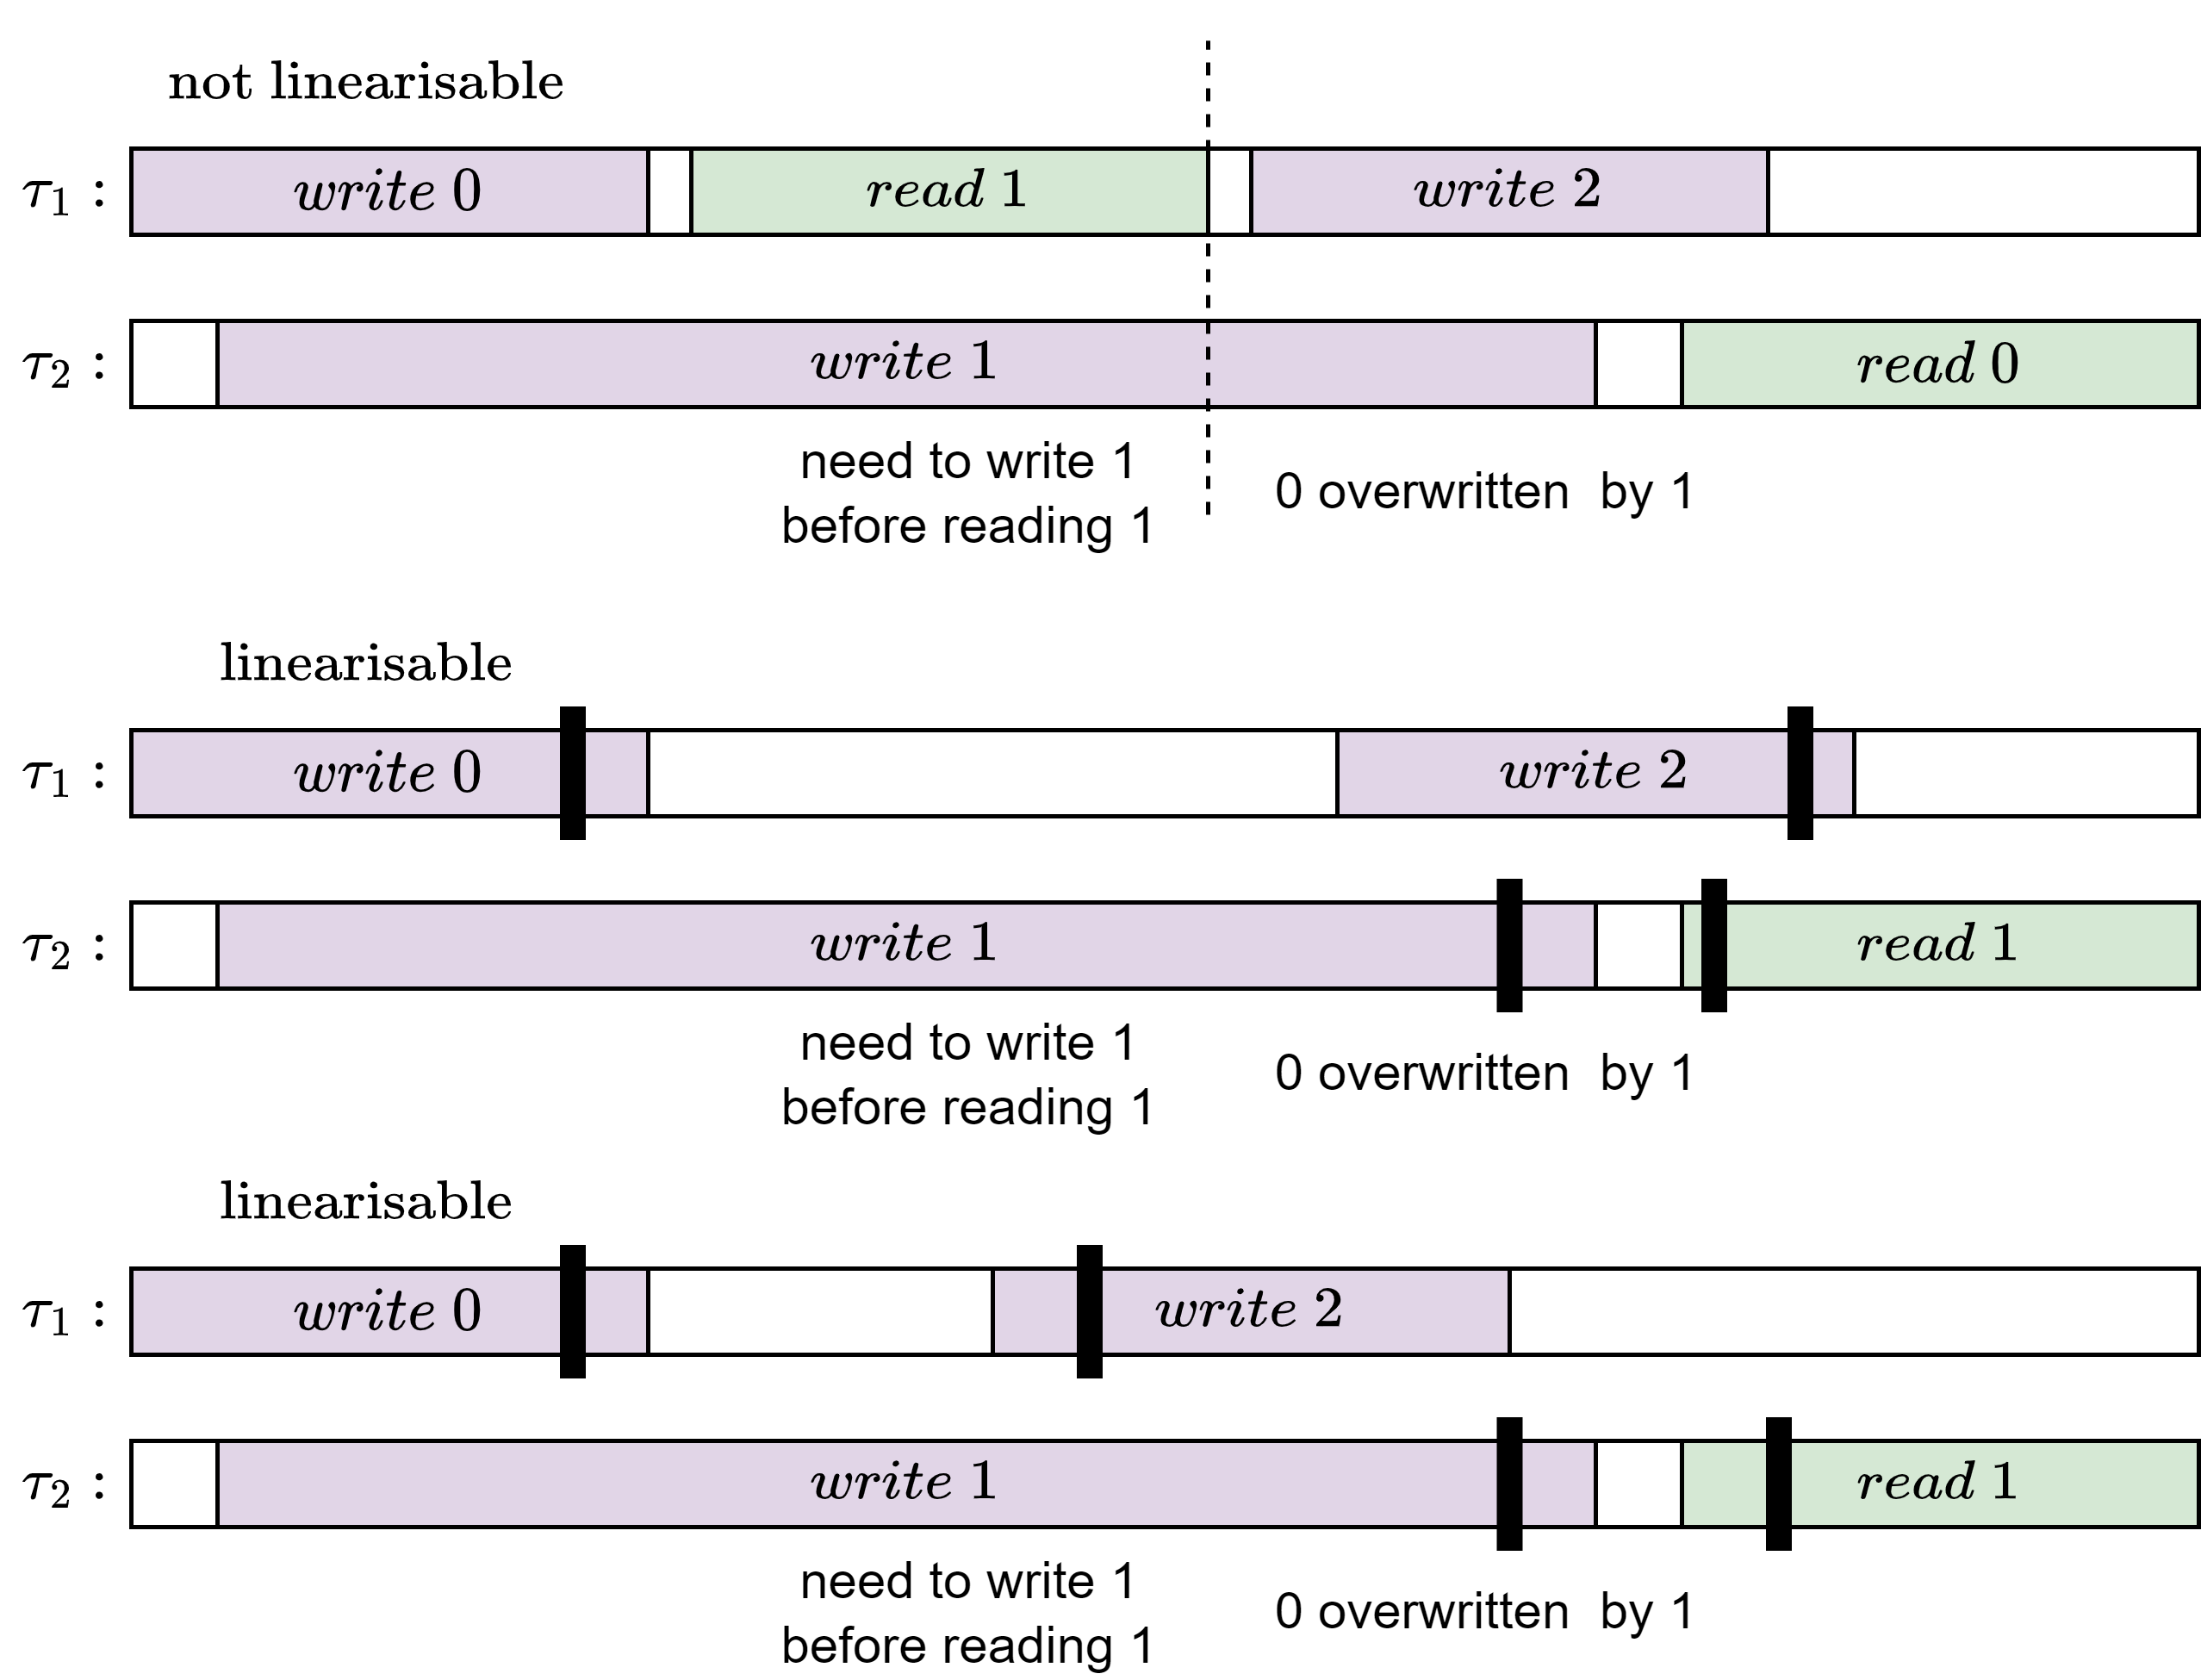
\includegraphics[width=.9\textwidth]{concurrent_objects/images/example_registers_linearisable_answer.drawio.png}
    \end{center}
\end{examplebox}

\section{Formal Model of Executions}

\begin{definitionbox}{Invocation and Response Notation}
    \[\left. \begin{matrix}
        \text{Invocation} \\
        Thread \quad object \ . \ method(args \dots) \\
    \end{matrix} \quad \right\lvert \quad \begin{matrix}
        \text{Response} \\
        Thread \quad object \ : \ return \\
    \end{matrix}\]
    \begin{itemize}
        \item Method name is implicit for response (a thread can only execute one method at once, so response directly follow's that thread's last invocation)
        \item An invocation is pending if there is no matching response
    \end{itemize}
\end{definitionbox}
\begin{definitionbox}{Histories}
    A history $H$ is a sequence of invocations and responses. For example:
    \[H = \begin{matrix*}[l]
        A & q.enq(7) \\
        B & p.enq(6) \\
        B & p : void \\
        B & q.deq() \\
        A & q: void \\
        B & q: 7 \\
    \end{matrix*}\]
    \[H|A = \begin{matrix*}[l]
        A & q.enq(7) \\
        A & q: void \\
    \end{matrix*} \qquad H|B = \begin{matrix*}[l]
        B & p.enq(6) \\
        B & p : void \\
        B & q.deq() \\
        B & q: 7 \\
    \end{matrix*} \qquad
    H|q = \begin{matrix*}[l]
        A & q.enq(7) \\
        B & q.deq() \\
        A & q: void \\
        B & q: 7 \\
    \end{matrix*} \qquad H|p = \begin{matrix*}[l]
        B & p.enq(6) \\
        B & p : void \\
    \end{matrix*}
    \]
    \begin{itemize}
        \item A history is \textit{well formed} if the per-thread projections are sequential.
        \item A history is \textit{sequential} if every invocations is immediately followed by its corresponding response.
        \item Histories are \textit{equivalent} if the per-thread projections are equivalent.
        \item A history is \textit{legal} if for every object $x$, $H|x$ is in the sequential spec for $x$.
    \end{itemize}
\end{definitionbox}

\begin{examplebox}{Equivalent Histories}
    Are $H$ and $G$ equivalent?
    \[H = \begin{matrix*}[l]
        A & q.enq(7) \\
        B & p.enq(6) \\
        B & p : void \\
        B & q.deq() \\
        A & q: void \\
        B & q: 7 \\
    \end{matrix*} \text{ and } G = \begin{matrix*}[l]
        B & p.enq(6) \\
        B & p : void \\
        A & q.enq(7) \\
        B & q.deq() \\
        B & q: 7 \\
        A & q: void \\
    \end{matrix*}\]
    \tcblower
    Yes, as $H|A = G|A$ and $H|B = G|B$.
\end{examplebox}
\begin{definitionbox}{Precedence}
    A method call $x$ precedes another $y$ if the response of $x$ is before the invocation of $y$. This is written as:
    \[\text{Given } H \quad m_0 \to_H m_1 \text{ if }m_0 \text{ precedes }m_1\]
    \begin{itemize}
        \item Precedence is a partial order (some methods overlap)
        \item For a fully sequential history, it is a total order.
    \end{itemize}
\end{definitionbox}


\section{Linearisability}
\begin{definitionbox}{Linearisability Formally}
    A history $H$ is linearisable if it can be extended to $G$ by:
    \begin{itemize}
        \item Appending zero or more responses to pending invocations.
        \item Discarding pending invocations.
    \end{itemize}
    Where $G$ will be equivalent to the \textit{legal sequential} history $S$ and ($\to_G \subseteq \to_S$)
\end{definitionbox}

\begin{definitionbox}{Composability Theorem}
    \[linearisable(H) \Leftrightarrow \forall x. \ [linearisable(H|x)]\]
    A history $H$ is linearisable if and only if for every object $x$, $H|x$ is linearisable.
    \begin{itemize}
        \item This allows for the linearisability of objects to be considered independently, and then composed.
    \end{itemize}
\end{definitionbox}
To show a history $H$ is linearisable:
\begin{enumerate}
    \item We can split the history using the composability theorem.
    \item Make the $H$ history complete (no pending invocations) (history $H'$)
    \item Create a sequential history $S$ that is legal (within sequential specification)
    \item Show $H'$ is equivalent to $S$ using projections.
    \item Get the strict total order $\to_S$ and show $\to_H$ is a subset of $\to_S$
\end{enumerate}


\section{Sequential Consistency}
A history $H$ is Sequentially Consistent if it can be extended to $G$ by:
\begin{itemize}
    \item Appending zero or more responses to pending invocations.
    \item Discarding pending invocations.
\end{itemize}
Where $G$ will be equivalent to the \textit{legal sequential} history $S$. Unlike with linearisability, $G$ does not have to be a subset of $S$.
